\documentclass[10pt]{article}
\usepackage[letterpaper,margin=0.6in]{geometry}
\usepackage{amsmath,amssymb,booktabs,array,graphicx}
\pagestyle{plain}\setlength{\parindent}{0pt}\setlength{\parskip}{3pt}
\allowdisplaybreaks\sloppy
\begin{document}
{\large\textbf{What ``hold $D/r$ fixed and let the octupole miss a little'' means (CoE model vs Migkas+2020 $A(\ell)$)}}\\[2pt]
Sedov--Taylor Center-of-Expansion model, analytic point-mass tidal form, sources on the vision shell ($d=r$), with Chris's rotation and $2\ell$ transforms.
Scripts: \texttt{figures/fixedDr\_octmiss.py} (solve + figure; reuses the data, coefficients and solver of \texttt{termmatch\_Dr234.py}) and \texttt{make\_fixedDr\_octmiss\_tex.py} (writes this sheet from \texttt{fixedDr\_octmiss\_results.json}).

\textbf{In one sentence.} With $D/r$ free, the four harmonic amplitudes ($m=0..3$) fix the four unknowns exactly and the octupole forces $D/r\approx1$. If we instead \emph{choose} $D/r=2,3,4$, we have one unknown fewer than equations; we match the mean, dipole and quadrupole, and the octupole amplitude becomes a \emph{prediction} that comes out too small. That shortfall is the ``miss''.

\medskip\textbf{Step 0. Chris's variables}\\
$r$ = vision-shell radius $=14.3$ Gpc; \ $D$ = our distance from the CoE; \ $L$ = density scale length; \ $M/M_0$ = enclosed mass toward the CoE (spreadsheet);
$(\ell_0,b_0)$ = longitude and tilt of the CoE axis; \ $\varphi$ = rotation phase in $\mathrm{Amp}_1\sin(\ell+\varphi)$; \ $\varphi_2$ = $2\ell$ phase in $\mathrm{Amp}_2\sin(2\ell+\varphi_2)$; \ Amp = harmonic amplitudes.

\medskip\textbf{Step 1. Define parameters}
\begin{align*}
&\varepsilon\equiv r/D=1/(D/r),\qquad M_{\rm crit}(<D)=\tfrac{4\pi}{3}\rho_cD^3=\frac{H_0^2D^3}{2G},\\
&\kappa\equiv\frac{G\,M(<D)}{H_0^2D^3}=\frac{M(<D)}{2M_{\rm crit}},\qquad K\equiv\alpha\kappa\ (\alpha=O(1);\ \text{tables use }\alpha=1),\\
&N=\text{overall normalisation},\qquad a\equiv\cos b_0,\qquad \mu=\cos b\cos b_0\cos\psi+\sin b\sin b_0,\qquad \psi=\ell-\ell_0 .
\end{align*}
Model, then averaged over the Migkas $90^\circ$ sectors ($|b|>20^\circ$, $\cos b$ weight; same coefficients as the v2 and term-matching sheets):
\begin{align*}
\frac{A}{A_{\rm all}}&=N\big[1+K(3\mu^2-1)+K\varepsilon(\tfrac92\mu-\tfrac{15}{2}\mu^3)\big]
\ \xrightarrow{\text{sector avg}}\ N(1+Kq_0)+NK\varepsilon\,o_1\cos\psi+NKq_2\cos2\psi+NK\varepsilon\,o_3\cos3\psi,\\
q_0&=0.4590-0.6885a^2,\quad q_2=0.49052a^2,\quad o_1=0.90032\,a(-3.1958+3.9948a^2),\quad o_3=-0.22806a^3 .
\end{align*}
$L$ does not appear: the point-mass form depends on the mass only through $K$, so $L$ (and $M/M_0$ separately from $L$) is not determined here.

\medskip\textbf{Step 2. Data harmonics and their $1\sigma$ errors}\\
Fourier fit to the 71 points ($m\le3$, $R^2=0.915$):
$A=0.9965+0.0296\cos\ell+0.0434\sin\ell+0.0636\cos2\ell+0.0366\sin2\ell-0.0299\cos3\ell-0.0114\sin3\ell$ (ordinary least squares; reproduced exactly).
Amplitudes $A_m=\sqrt{a_m^2+b_m^2}$ with $\sigma_{A_m}^2=g^{T}\,\mathrm{Cov}(a_m,b_m)\,g$, $g=(a_m,b_m)/A_m$. The coefficient covariance is computed three ways:
\begin{itemize}\setlength{\itemsep}{0pt}
\item[(i)] \emph{naive}: 71 independent points, $\sigma_i=(\sigma_{\rm lo}+\sigma_{\rm hi})/2$, $\mathrm{Cov}=(X^TWX)^{-1}$ (the weights used in the earlier sheets);
\item[(ii)] \emph{$N_{\rm eff}=16$}: (i)$\times\sqrt{71/16}$ (rule of thumb: $\sim$16 independent sectors);
\item[(iii)] \emph{sector-correlated} (adopted): $\mathrm{Cov}=B\,C\,B^T$, $B=(X^TX)^{-1}X^T$, $C_{ij}=\sigma_i\sigma_j\max(0,\,1-|\ell_i-\ell_j|/90^\circ)$, the overlap fraction of two $90^\circ$ sectors when clusters are uniform on the sky.
\end{itemize}
Model (iii) is supported by the residuals: their rms about the $m\le3$ fit is $0.021$, versus a mean error bar of $0.097$ (naive $\chi^2/\nu=0.05$). That is impossible for independent points, and it is what boxcar-smoothed noise predicts. The smoothing damps high $m$ strongly, so (iii) gives a large error on $A_1$ and a small one on $A_3$.
\begin{center}\small
\begin{tabular}{lcccc}\toprule
 & $A_0$ & $A_1$ (peak $55.7^\circ$) & $A_2$ (peak $14.96^\circ$) & $A_3$ (peak $67.0^\circ$)\\\midrule
value & $0.9965$ & $0.0525$ & $0.0734$ & $0.0320$\\
$\sigma$ (iii) sector-correlated & $0.0489$ & $0.0602$ & $0.0439$ & $0.0212$\\
$\sigma$ (ii) $N_{\rm eff}=16$ & $0.0242$ & $0.0329$ & $0.0336$ & $0.0331$\\
$\sigma$ (i) naive & $0.0115$ & $0.0156$ & $0.0160$ & $0.0157$\\
signal/$\sigma_{\rm (iii)}$ & -- & $0.87$ & $1.67$ & $1.51$\\\bottomrule
\end{tabular}
\end{center}
Under (iii), the amplitude estimates are mildly correlated ($|\rho|\le0.26$); the $\chi^2$ below ignores that. Even the octupole itself is only a $1.5\sigma$ feature.

\medskip\textbf{Step 3. Set amplitudes equal, then count equations and unknowns}\\
With $P\equiv NK$ and the axis fixed at the quadrupole peak, $\ell_0=\ell_2=14.96^\circ$:
\[
\text{(E0)}\ N(1+Kq_0)=A_0,\qquad \text{(E1)}\ P\varepsilon|o_1|=A_1,\qquad \text{(E2)}\ P\,q_2=A_2,\qquad \text{(E3)}\ P\varepsilon|o_3|=A_3 .
\]
\emph{Free $\varepsilon$:} unknowns $N,K,b_0,\varepsilon$ $\Rightarrow$ 4 equations, 4 unknowns: an exact solve with nothing left over to test.\\
\emph{Fixed $D/r$:} $\varepsilon$ is given, so there are 3 unknowns $N,K,b_0$ but still 4 equations: overdetermined by one.
$N$ appears only in (E0), which is therefore satisfied exactly by $N=A_0-Pq_0$. That leaves (E1)--(E3), three equations in $(P,b_0)$, so one degree of freedom is left to test.

\medskip\textbf{Step 4. Which ratio pins $\varepsilon$}\\
Divide the equations so that $P$ cancels:
\[
\frac{A_3}{A_1}=\frac{|o_3|}{|o_1|}\ \ (\varepsilon\text{ cancels: fixes }b_0\text{ only}),\qquad
\frac{A_1}{A_2}=\varepsilon\,\frac{|o_1|}{q_2},\qquad
\frac{A_3}{A_2}=\varepsilon\,\frac{|o_3|}{q_2}=\varepsilon\,\frac{0.22806a^3}{0.49052a^2}=0.46494\,a\,\varepsilon .
\]
The dipole and octupole \emph{both} carry $\varepsilon$, so $A_3/A_1$ says nothing about $\varepsilon$. The octupole-to-quadrupole ratio does, and it has a very simple form. Since $a=\cos b_0\le1$:
\[
\varepsilon=\frac{A_3/A_2}{0.46494\,a}\ \ge\ \frac{0.4361}{0.46494}=0.9379\qquad\Longrightarrow\qquad D/r\le1.066\quad\text{(central values).}
\]
Read the other way round: if (E2) is matched, the octupole the model can produce is capped at $A_3^{\rm pred}\le0.46494\,\varepsilon\,A_2$. That cap is
$0.0171, 0.0114, 0.0085$ for $D/r=2,3,4$, against the data value $0.0320$.
\emph{Fixing $\varepsilon$ smaller than $0.938$ therefore forces the predicted octupole below the data, whatever $b_0$ is.}

\emph{Free-$\varepsilon$ solve (check).} $A_3/A_1=0.6091=|o_3/o_1|$ gives $b_0=19.10^\circ$ ($a=0.94496$; on-axis dipole) or $31.66^\circ$ (flipped dipole). Then
$P=A_2/q_2=0.07338/0.43801=0.16753$ and $\varepsilon=A_3/(P|o_3|)=0.99257$ ($D/r=1.0075$),
$N=A_0-Pq_0=1.02260$, $K=P/N=0.16383$. The flipped root gives $\varepsilon=1.1019$ ($D/r=0.9075$), $K=0.2055$. Both reproduce the old v2 sheet.

\medskip\textbf{Step 5. The least-squares objective at fixed $\varepsilon$}
\[
\chi^2(P,b_0;\varepsilon)=\sum_{m=1}^{3}\frac{\big(A_m-P\,c_m(b_0,\varepsilon)\big)^2}{\sigma_m^2},\qquad c_1=\varepsilon|o_1|,\ c_2=q_2,\ c_3=\varepsilon|o_3|,\qquad
P(b_0)=\frac{\sum_m A_mc_m/\sigma_m^2}{\sum_m c_m^2/\sigma_m^2},
\]
and $\chi^2(b_0)$ is minimised by a $0.05^\circ$ scan plus a bounded 1-D refinement. Two recipes are used:
\textbf{(LSQ)} weights $1/\sigma_m^2$ from (i). These are the weights of the earlier term-matching run, and they are nearly equal, so the absolute scale does not matter.
\textbf{(Exact)} solve (E0)--(E2) exactly and treat (E3) as a pure prediction. From $A_1/A_2=\varepsilon|o_1|/q_2$ we get $b_0$, then $P=A_2/q_2$, and $A_3^{\rm pred}=0.46494\,a\,\varepsilon A_2$.
Because the dipole and quadrupole are then matched exactly, every bit of misfit goes into $A_3$.
In both recipes the misses are quoted as pulls $(A^{\rm pred}_m-A_m)/\sigma_m$ under each error model. The phases are Chris's transforms: $\phi_1=\ell_1^{\rm data}-\ell^{(1)}_{\rm nat}$ (rotation), $\phi_2=0$ (the $2\ell$ phase is set by $\ell_0$), and the octupole stays at its natural peak $\ell_0+60^\circ$, i.e.\ $\delta_3=-8.00^\circ$ from the data.
$R^2$ is that of the transformed curve against the 71 points.


\medskip\textbf{Step 6. Solve at $D/r=2,3,4$: predicted harmonics vs data}
\begin{center}\footnotesize\setlength{\tabcolsep}{3.0pt}
\begin{tabular}{lcccccccccccc}\toprule
 & & & & \multicolumn{3}{c}{predicted amplitude} & \multicolumn{4}{c}{pull $=(\text{pred}-\text{data})/\sigma$} & & \\\cmidrule(lr){5-7}\cmidrule(lr){8-11}
case & $b_0$ & $N$ & $K$ & $A_1$ & $A_2$ & $A_3$ & $A_1,A_2$ (iii) & $A_3$ (iii) & $A_3$ (ii) & $A_3$ (i) & $\chi^2_{\rm (iii)}$ & $R^2$\\\midrule
data $\pm\sigma_{\rm (iii)}$ & & & & $0.0525$ & $0.0734$ & $0.0320$ & & & & & & $0.915^{a}$\\
 & & & & $\pm0.060$ & $\pm0.044$ & $\pm0.021$ & & & & & & \\\midrule

free $\varepsilon$, $D/r=1.0075$ & $19.1^\circ$ & $1.0226$ & $0.1638$ & $0.0525$ & $0.0734$ & $0.0320$ & $+0.00$, $+0.00$ & $+0.00$ & $+0.00$ & $+0.00$ & $0.00$ & $0.897$\\
$D/r=2$ LSQ & $6.3^\circ$ & $1.0314$ & $0.1529$ & $0.0530$ & $0.0764$ & $0.0177$ & $+0.01$, $+0.07$ & $-0.68$ & $-0.43$ & $-0.91$ & $0.46$ & $0.884$\\
$D/r=3$ LSQ & $40.0^\circ$ & $0.9820$ & $0.2708$ & $0.0519$ & $0.0766$ & $0.0091$ & $-0.01$, $+0.07$ & $-1.08$ & $-0.69$ & $-1.46$ & $1.17$ & $0.858$\\
$D/r=4$ LSQ & $43.3^\circ$ & $0.9688$ & $0.3025$ & $0.0519$ & $0.0761$ & $0.0064$ & $-0.01$, $+0.06$ & $-1.21$ & $-0.77$ & $-1.63$ & $1.46$ & $0.846$\\
\midrule

$D/r=2$ exact, on-axis & $4.1^\circ$ & $1.0305$ & $0.1459$ & $0.0525$ & $0.0734$ & $0.0170$ & $-0.00$, $+0.00$ & $-0.71$ & $-0.45$ & $-0.95$ & $0.50$ & $0.884$\\
$D/r=2$ exact, flipped & $36.7^\circ$ & $0.9928$ & $0.2342$ & $0.0525$ & $0.0734$ & $0.0137$ & $+0.00$, $+0.00$ & $-0.86$ & $-0.55$ & $-1.17$ & $0.75$ & $0.875$\\
$D/r=3$ exact, flipped & $40.5^\circ$ & $0.9806$ & $0.2642$ & $0.0525$ & $0.0734$ & $0.0086$ & $+0.00$, $+0.00$ & $-1.10$ & $-0.71$ & $-1.49$ & $1.22$ & $0.856$\\
$D/r=4$ exact, flipped & $43.9^\circ$ & $0.9671$ & $0.2982$ & $0.0525$ & $0.0734$ & $0.0061$ & $+0.00$, $+0.00$ & $-1.22$ & $-0.78$ & $-1.65$ & $1.49$ & $0.846$\\
\midrule

$D/r=3$ LSQ, $b_0{=}0$ branch & $0.0^\circ$ & $1.0352$ & $0.1628$ & $0.0404$ & $0.0826$ & $0.0128$ & $-0.20$, $+0.21$ & $-0.91$ & $-0.58$ & $-1.22$ & $0.91$ & $0.848$\\
$D/r=4$ LSQ, $b_0{=}0$ branch & $0.0^\circ$ & $1.0360$ & $0.1659$ & $0.0309$ & $0.0843$ & $0.0098$ & $-0.36$, $+0.25$ & $-1.05$ & $-0.67$ & $-1.41$ & $1.29$ & $0.801$\\
\bottomrule
\end{tabular}\\[2pt]
{\footnotesize $^a$Fourier fit, octupole at its own phase. \ ``on-axis''/``flipped'' = sign of $o_1$ (dipole natural peak at $\ell_0$ or $\ell_0+180^\circ$).
At $D/r\ge2.05$ the on-axis branch can no longer reach $A_1/A_2$ (its maximum of $\varepsilon|o_1|/q_2$ is $1.4665\,\varepsilon$ at $b_0=0$), so the exact recipe has only the flipped root there.}
\end{center}

\textbf{What the table says.} In every fixed-$D/r$ row the dipole and quadrupole are reproduced to within $0.1\sigma$ (LSQ) or exactly (exact recipe); the whole cost sits in the octupole.
The predicted $A_3$ falls roughly as $\varepsilon$: $0.0177, 0.0091, 0.0064$ at $D/r=2,3,4$, against $0.0320$.
That is a miss of $0.7, 1.1, 1.2\,\sigma$ with the adopted errors ((ii): $0.4, 0.7, 0.8\,\sigma$; naive (i): $0.9, 1.5, 1.6\,\sigma$).
$R^2$ drops from $0.897$ to $0.884, 0.858, 0.846$. The curves themselves differ by little more than a $3\ell$ ripple of amplitude $\lesssim0.032$ (Fig.~1c,d).
This is the precise meaning of ``the octupole misses a little'': a $\sim$1--1.6$\sigma$ shortfall in one harmonic that is itself only a $1.5\sigma$ detection.

\textbf{How much can the octupole constrain $D/r$?} The profile $\chi^2_{\rm (iii)}(D/r)$, minimised over $(P,b_0)$ with weights (iii) (one degree of freedom), is
$0.42, 0.89, 1.28, 1.75$ at $D/r=2,3,4,6$, with minimum $\approx0$ at $D/r\approx1$.
$\Delta\chi^2=1$ is crossed at $D/r\approx3.28$ and $\Delta\chi^2=4$ is never reached: as $\varepsilon\to0$, $\chi^2\to(A_3/\sigma_3)^2=2.28$.
With the naive errors (i) the corresponding numbers are $\Delta\chi^2=1$ at $D/r\approx2.16$ and an asymptote of $(A_3/\sigma_3)^2=4.16$.
So the central values prefer $D/r\approx1$, but the octupole alone cannot exclude $D/r=2$--$4$ at even $2\sigma$ under any of the three error models.
With the (iii) weights the LSQ optimum at $D/r=3$ and $4$ switches to the $b_0=0$ branch ($\chi^2_{\rm (iii)}=0.89, 1.28$), so the $b_0$ reported at those $D/r$ is weight-dependent. The $A_3$ shortfall is not.


\begin{figure}[!htbp]\centering
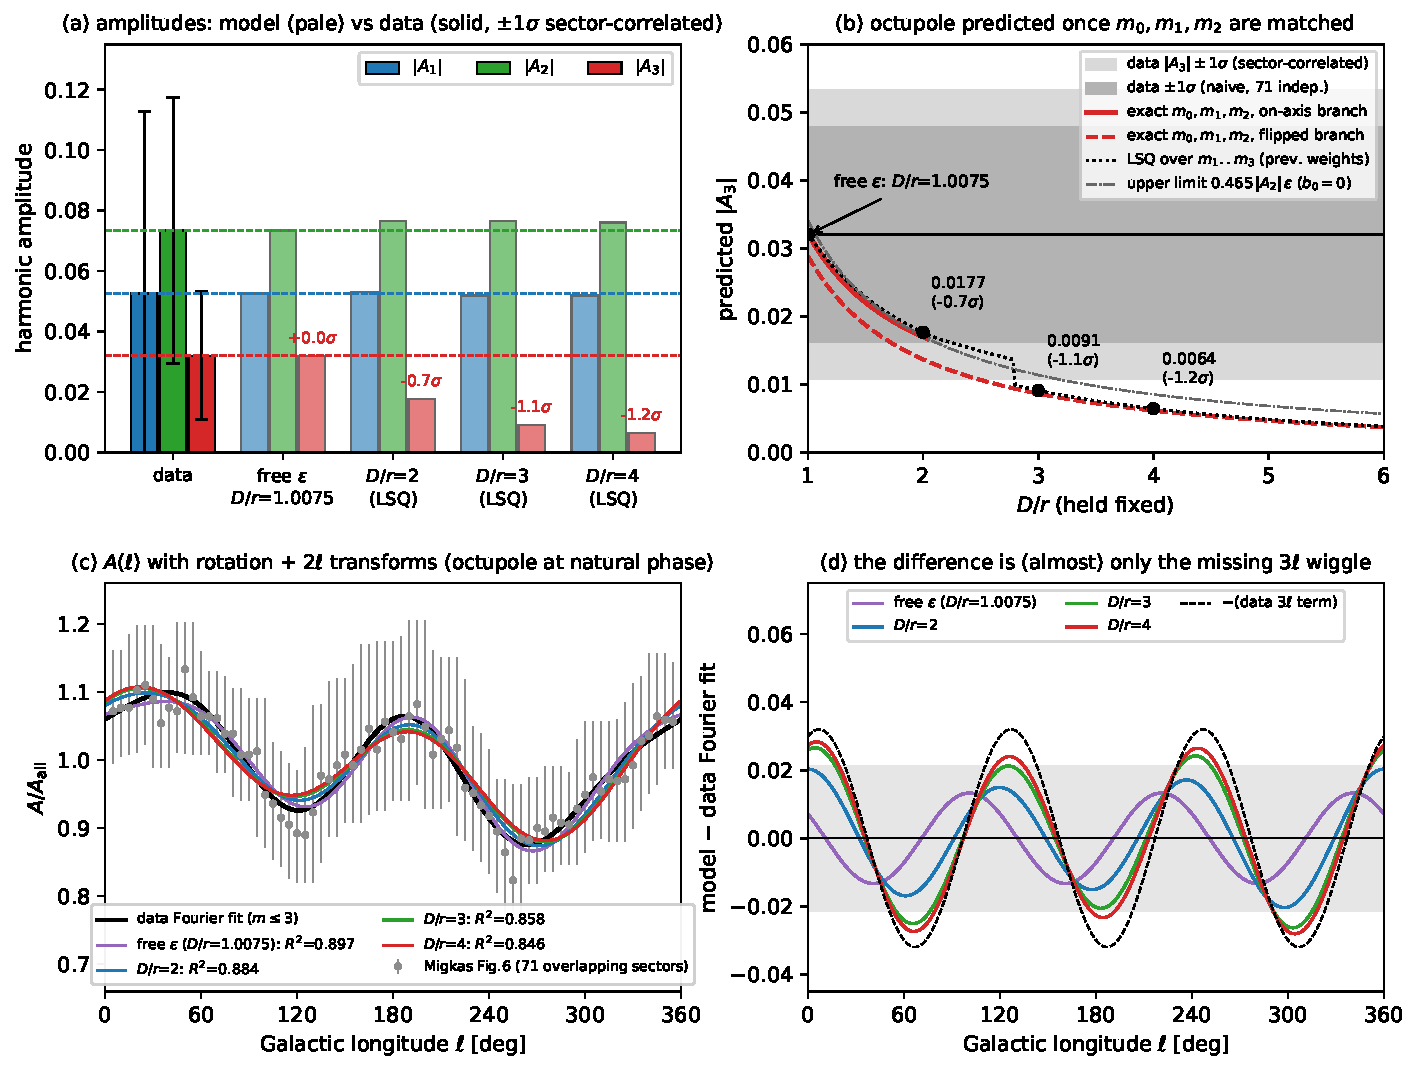
\includegraphics[width=0.74\textwidth]{../../figures/fixedDr_octmiss.pdf}
\caption{\small (a) Harmonic amplitudes: data with $\pm1\sigma$ (iii) error bars, and the model at free $\varepsilon$ and at $D/r=2,3,4$ (LSQ). The octupole pull is written above each red bar.
(b) Predicted octupole vs the fixed $D/r$ once $m_0$--$m_2$ are fitted: exact recipe (solid: on-axis branch, which exists up to $D/r=2.05$; dashed: flipped branch), LSQ (dotted; the step at $D/r\approx2.8$ is the switch from the on-axis to the flipped minimum), and the cap $0.465\,\varepsilon A_2$.
The curve meets the data at $D/r=1.0075$, the free-$\varepsilon$ solution. Grey bands: data $\pm1\sigma$ (light: (iii); dark: naive (i)).
(c) $A(\ell)$: the 71 digitised points, the Fourier fit, and the transformed model curves. (d) Model minus Fourier fit: at fixed $D/r$ the residual is almost a pure $3\ell$ wave, close to minus the data's octupole term.
The free-$\varepsilon$ residual is the $\delta_3=-8^\circ$ octupole phase offset. Shaded: $\pm\sigma_3$ (iii).}
\end{figure}


\medskip\textbf{Step 7. Back to Chris's variables} (LSQ solutions of Step 6; $r=14.3$ Gpc, $\alpha=1$)
\begin{center}\small
\begin{tabular}{lcccc}\toprule
 & free $\varepsilon$ & $D/r=2$ & $D/r=3$ & $D/r=4$\\\midrule

$D/r$ & $1.0075$ & $2.0000$ & $3.0000$ & $4.0000$\\
$D=14.3\,$Gpc$\times D/r$: Gpc (Gly) & $14.41$ ($47.0$) & $28.60$ ($93.3$) & $42.90$ ($139.9$) & $57.20$ ($186.6$)\\
$K=\alpha\kappa$; \ $M(<D)/M_{\rm crit}=2K/\alpha$ & $0.1638$; $0.328$ & $0.1529$; $0.306$ & $0.2708$; $0.542$ & $0.3025$; $0.605$\\
$N$ & $1.0226$ & $1.0314$ & $0.9820$ & $0.9688$\\
tilt $b_0$ (dipole branch) & $19.10^\circ$ (on-axis) & $6.26^\circ$ (on-axis) & $39.96^\circ$ (flipped) & $43.32^\circ$ (flipped)\\
$\ell_0$ & $14.96^\circ$ & $14.96^\circ$ & $14.96^\circ$ & $14.96^\circ$\\
rotation $\phi_1$ & $+40.75^\circ$ & $+40.75^\circ$ & $-139.25^\circ$ & $-139.25^\circ$\\
Chris's $\varphi$ (model$\to$data) & $75.0\to34.30^\circ$ & $75.0\to34.30^\circ$ & $-105.0\to34.30^\circ$ & $-105.0\to34.30^\circ$\\
$2\ell$ phase $\phi_2$; \ $\varphi_2$ & $0^\circ$; $60.08^\circ$ & $0^\circ$; $60.08^\circ$ & $0^\circ$; $60.08^\circ$ & $0^\circ$; $60.08^\circ$\\
Amp$_1$, Amp$_2$ & $0.0525$, $0.0734$ & $0.0530$, $0.0764$ & $0.0519$, $0.0766$ & $0.0519$, $0.0761$\\
Amp$_3$ (predicted) vs $0.0320$ & $0.0320$ ($+0.0\sigma$) & $0.0177$ ($-0.7\sigma$) & $0.0091$ ($-1.1\sigma$) & $0.0064$ ($-1.2\sigma$)\\
octupole phase offset $\delta_3$ & $-8.0^\circ$ & $-8.0^\circ$ & $-8.0^\circ$ & $-8.0^\circ$\\
\bottomrule
\end{tabular}
\end{center}
$\varphi$ and $\varphi_2$ are identical in all columns. The transforms put the dipole and quadrupole peaks on the data by construction, so only the amplitudes and $b_0$ carry information about $D/r$.
$L$ and $M/M_0$ are not separately determined by this analytic form; only $K\propto M(<D)/D^3$ enters.


\textbf{Caveats.} (1) Chris's rotation $\phi_1\approx41^\circ$ and the choice $\ell_0=\ell_2$ are extra phase freedom that the axisymmetric physics does not predict; the test here is on amplitudes only.
(2) The analytic form is an $O(\varepsilon)$ tidal expansion, and the preferred solution sits at $\varepsilon\approx1$, where that expansion is not reliable. The bound $\varepsilon\ge0.938$ is a statement about this truncated form.
(3) Error model (iii) assumes uniform clusters and purely statistical, sector-overlap-correlated error bars read from a digitised figure; the true $\sigma_m$ could differ by tens of percent. Model (ii) gives $\sigma_3$ about $1.6\times$ larger, and model (i) about $1.35\times$ smaller.
(4) The sector coefficients $q,o$ assume a uniform sky outside $|b|\le20^\circ$; the real cluster distribution will shift them, and hence the $0.465$ in the cap.
(5) All earlier fixed-$D/r$ numbers (termmatch\_Dr234: $N,K,b_0,R^2$, analytic octupole $0.0177,\ 0.0091,\ 0.0064$) are reproduced to machine precision. The previously quoted pulls used the naive errors (i).
\end{document}
